\documentclass[12pt,a4paper]{article}
\usepackage[utf8]{inputenc}
\usepackage[T1]{fontenc}
\usepackage[brazil]{babel}
\usepackage[a4paper,margin=2.3cm]{geometry}
\usepackage{booktabs,array,enumitem,hyperref,tikz,float,listings,xcolor,graphicx,longtable,caption}
\usetikzlibrary{positioning}
\hypersetup{hidelinks}
\setlength{\parindent}{1.5em}
\lstset{basicstyle=\ttfamily\footnotesize,frame=single,breaklines=true,backgroundcolor=\color{black!4},columns=fullflexible}
\renewcommand{\arraystretch}{1.12}
\newcommand{\cod}[1]{\texttt{#1}}

\begin{document}
\begin{titlepage}
\centering
{\large UNIVERSIDADE FEDERAL DO PARÁ (UFPA)}\\[0.3cm]
{\large INSTITUTO DE CIÊNCIAS EXATAS E NATURAIS (ICEN)}\\[0.3cm]
{\large CURSO DE CIÊNCIA DA COMPUTAÇÃO}\\[1cm]
{\large Laboratório de Sistemas Distribuídos}\\[3cm]
{\LARGE\bfseries RELATÓRIO DETALHADO DE ARQUITETURA DE REDE}\\[0.6cm]
{\large Cenário 2 -- Equipe 8\\ WAN com núcleo em malha completa, OSPF área 0 e RIP em paralelo}\\[1cm]
{\normalsize Arquivo analisado: \texttt{cenario2\_equipe8\_lab\_SD.pkt}\\ Cisco Packet Tracer 9.0.1.0858}\\[3cm]
\vfill
{\large Belém - PA}\\[0.2cm]{\large Outubro de 2026}
\end{titlepage}

\tableofcontents
\newpage

%=====================================================================
\section{Introdução, fonte dos dados e metodologia}
Este relatório descreve, em nível de camada física, enlace, rede e serviços, a arquitetura contida em \texttt{cenario2\_equipe8\_lab\_SD.pkt}. O arquivo é um contêiner cifrado do Packet Tracer; o notebook \texttt{ferramentas/pkt\_decrypt.ipynb} (Twofish-EAX, \textit{de-obfuscation} posicional e \texttt{qCompress}) foi usado para recuperar o XML da topologia (1\,301\,981 bytes, versão \texttt{9.0.1.0858}).

\paragraph{O que foi extraído.} Do XML foram lidos programaticamente: os 22 dispositivos (módulos, portas, largura de banda), os 23 cabos (\texttt{LINKS}), as \textit{running-configs} de roteadores e switches, o estado de DHCP dos PCs e o \textbf{histórico de comandos de CLI} (\texttt{COMMAND\_LOGS}, 898 entradas). A imagem do cenário real, exportada do espaço lógico do Packet Tracer (\texttt{cenario\_real.png}), foi usada para conferir a disposição dos dispositivos.

\paragraph{O que foi calculado.} Tabelas de roteamento esperadas, caminhos mais curtos, custos OSPF e análise de falhas foram \textbf{calculados} a partir da topologia, das larguras de banda gravadas e das regras padrão do OSPF (custo $=\lfloor 10^8 / bw_{bps}\rfloor$, mínimo 1). Não vieram de uma simulação em execução. Esses itens estão marcados como \textit{esperados} e devem ser confirmados no Packet Tracer (Seção~\ref{sec:testes}).

\paragraph{Limitação.} O arquivo guarda o estado \textbf{salvo}. Concessões DHCP, tabelas ARP, vizinhanças OSPF e rotas aprendidas não são persistidas, então o estado operacional não pode ser lido diretamente.

%=====================================================================
\section{Visão geral e inventário}
A rede interliga \textbf{quatro LANs} por um \textit{backbone} WAN de \textbf{quatro roteadores de núcleo} (R0--R3) em \textbf{malha completa} (6 enlaces seriais). Cada LAN é atendida por um roteador de borda (R4--R7), ligado por um enlace serial a exatamente um roteador de núcleo. O roteamento é dinâmico: \textbf{OSPF processo 1, área única 0}.

\begin{table}[H]\centering\small
\begin{tabular}{@{}lr@{}}\toprule
Dispositivos no arquivo & 22 (8 roteadores, 4 switches, 9 PCs, 1 \textit{Power Distribution Device} sem cabos)\\
Roteadores (núcleo / borda) & 8 (4 / 4), modelo \textit{Router-PT-Empty}\\
Switches & 4, modelo \textit{Switch-PT-Empty} (4 portas GigabitEthernet cada)\\
Estações & 9 \textit{PC-PT} (1 porta FastEthernet)\\
Cabos & 23: 10 seriais + 13 de cobre \textit{straight-through}\\
Todos os cabos funcionais & sim (\texttt{FUNCTIONAL=true} nos 23)\\
Domínios de \textit{broadcast} & 14 (4 LANs + 10 enlaces ponto a ponto)\\
Sub-redes & 14: 4 LANs \texttt{/24} + 10 enlaces WAN \texttt{/16}\\
Área OSPF / processo & 0 / 1\\ \bottomrule
\end{tabular}
\caption{Inventário do cenário.}
\end{table}

\subsection{Módulos de hardware}
\begin{itemize}[nosep]
\item \textbf{R0--R3 (núcleo):} 4 módulos \texttt{PT-ROUTER-NM-1SS} (serial inteligente), portas \texttt{Serial6/0} a \texttt{Serial9/0}. Não possuem interface LAN.
\item \textbf{R4--R7 (borda):} \texttt{PT-ROUTER-NM-1S} (\texttt{Serial0/0}) e \texttt{PT-ROUTER-NM-1CGE} (\texttt{GigabitEthernet9/0}).
\item \textbf{Switches:} 4 $\times$ \texttt{PT-SWITCH-NM-1CGE}: \texttt{Gi0/1}, \texttt{Gi7/1}, \texttt{Gi8/1}, \texttt{Gi9/1}.
\item \textbf{PCs:} \texttt{PT-HOST-NM-1CFE} (FastEthernet0, 100 Mb/s) mais uma interface Bluetooth desligada.
\end{itemize}

%=====================================================================
\section{Topologia}
\begin{figure}[H]\centering
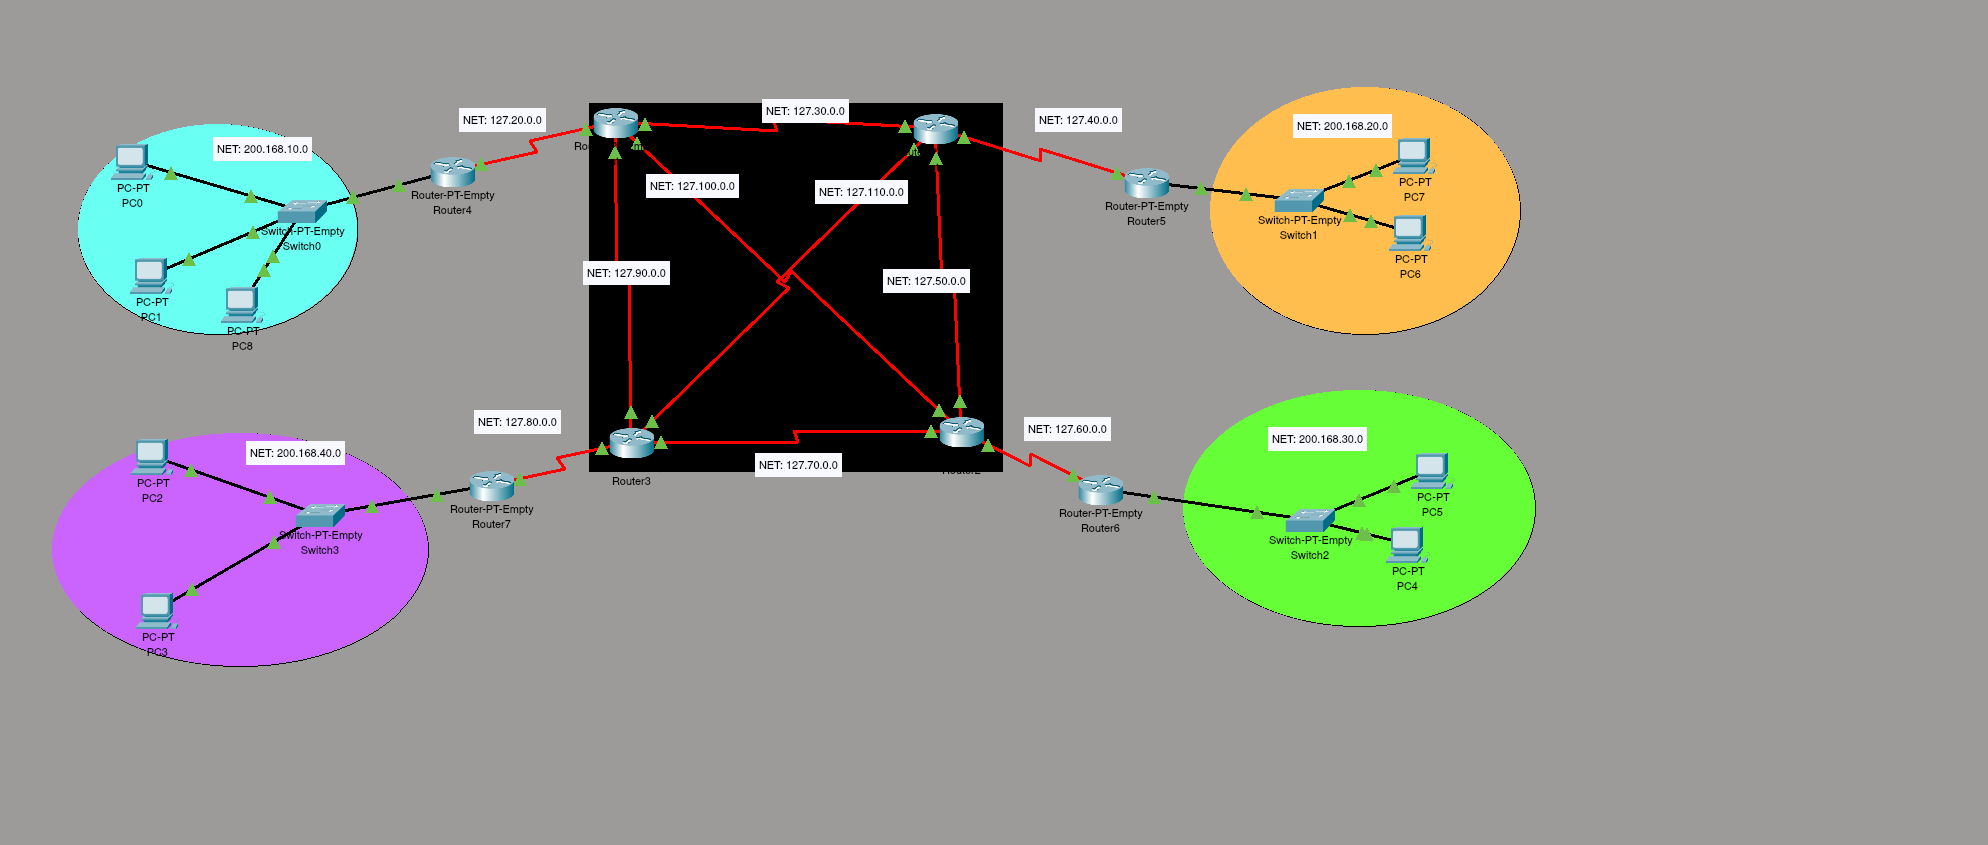
\includegraphics[width=\linewidth,trim=30 131 328 56,clip]{cenario_real.png}
\caption{Cenário real montado no Packet Tracer (espaço lógico). Elipses coloridas: LANs; retângulo preto: núcleo; os rótulos \texttt{NET:} são anotações do projetista. Os rótulos dos enlaces mostram \texttt{127.x.0.0}, mas as interfaces configuradas usam \texttt{172.x.0.0} (ver Seção~\ref{sec:auditoria}).}
\end{figure}

\begin{figure}[H]\centering
\begin{tikzpicture}[
 r/.style={circle,draw,thick,minimum size=9mm,inner sep=0,font=\small\bfseries,fill=yellow!25},
 e/.style={circle,draw,thick,minimum size=9mm,inner sep=0,font=\small\bfseries,fill=blue!10},
 s/.style={rectangle,draw,minimum width=9mm,minimum height=5mm,font=\scriptsize,fill=green!15},
 w/.style={thick,red!70!black},
 l/.style={font=\tiny,fill=white,inner sep=1pt}]
\node[r] (r0) at (0,3) {R0};
\node[r] (r1) at (5,3) {R1};
\node[r] (r2) at (5,0) {R2};
\node[r] (r3) at (0,0) {R3};
\draw[w] (r0) -- node[l]{172.30/16} (r1);
\draw[w] (r1) -- node[l,pos=.3]{172.50/16} (r2);
\draw[w] (r2) -- node[l]{172.70/16} (r3);
\draw[w] (r3) -- node[l,pos=.3]{172.90/16} (r0);
\draw[w] (r0) -- node[l,pos=.28]{172.100/16} (r2);
\draw[w] (r3) -- node[l,pos=.28]{172.110/16} (r1);
\node[e] (r4) at (-3.5,3) {R4};
\node[e] (r5) at (8.5,3) {R5};
\node[e] (r6) at (8.5,0) {R6};
\node[e] (r7) at (-3.5,0) {R7};
\draw[w] (r4) -- node[l]{172.20/16} (r0);
\draw[w] (r5) -- node[l]{172.40/16} (r1);
\draw[w] (r6) -- node[l]{172.60/16} (r2);
\draw[w] (r7) -- node[l]{172.80/16} (r3);
\node[s] (s0) at (-3.5,4.7) {Switch0}; \draw (r4)--(s0);
\node[s] (s1) at (8.5,4.7) {Switch1}; \draw (r5)--(s1);
\node[s] (s2) at (8.5,-1.7) {Switch2}; \draw (r6)--(s2);
\node[s] (s3) at (-3.5,-1.7) {Switch3}; \draw (r7)--(s3);
\node[font=\scriptsize,align=center] at (-3.5,5.7) {PC0, PC1, PC8\\200.168.10.0/24};
\node[font=\scriptsize,align=center] at (8.5,5.7) {PC6, PC7\\200.168.20.0/24};
\node[font=\scriptsize,align=center] at (8.5,-2.7) {PC4, PC5\\200.168.30.0/24};
\node[font=\scriptsize,align=center] at (-3.5,-2.7) {PC2, PC3\\200.168.40.0/24};
\node[font=\scriptsize,yellow!40!black] at (2.5,1.5) {\textbf{Núcleo OSPF}};
\end{tikzpicture}
\caption{Topologia reconstruída a partir do XML. Amarelo: núcleo; azul: borda.}
\end{figure}

\subsection{Camadas funcionais}
\begin{description}[leftmargin=1.5em]
\item[Acesso.] PCs $\to$ switch (100 Mb/s) $\to$ \texttt{Gi9/0} do roteador de borda (1 Gb/s), que é o \textit{gateway} \texttt{.254} da LAN.
\item[Borda.] R4--R7 têm uma serial (T1, 1544 kb/s) para o núcleo. Cada site depende de um único enlace de acesso e de um único roteador.
\item[Núcleo.] R0--R3 formam um $K_4$: os 6 pares possuem enlace direto. Para qualquer par de núcleos há 3 caminhos disjuntos em enlaces (direto e via cada um dos outros dois).
\end{description}

\subsection{Mapeamento borda--núcleo--LAN}
\begin{table}[H]\centering\small
\begin{tabular}{@{}llllll@{}}\toprule
Borda & Núcleo de acesso & Rede de acesso & LAN & Rótulo (descrição) & Switch\\\midrule
R4 & R0 & 172.20.0.0/16 & 200.168.10.0/24 & LAN-SiteA & Switch0\\
R5 & R1 & 172.40.0.0/16 & 200.168.20.0/24 & LAN-SiteC & Switch1\\
R6 & R2 & 172.60.0.0/16 & 200.168.30.0/24 & LAN-SiteD & Switch2\\
R7 & R3 & 172.80.0.0/16 & 200.168.40.0/24 & LAN-SiteB & Switch3\\\bottomrule
\end{tabular}
\caption{As letras A--D vêm das \texttt{description} das interfaces e não seguem a ordem R4--R7: o Site B é o de R7 e o Site C o de R5.}
\end{table}

%=====================================================================
\section{Camada física e enlace}
\subsection{Enlaces seriais}
\begin{table}[H]\centering\small
\begin{tabular}{@{}lllllll@{}}\toprule
Rede & Extremo A & IP A & Extremo B & IP B & Lado DCE\\\midrule
172.30.0.0/16 & R0 S6/0 & .1 & R1 S6/0 & .2 & R0\\
172.50.0.0/16 & R1 S7/0 & .1 & R2 S7/0 & .2 & R1\\
172.70.0.0/16 & R2 S8/0 & .1 & R3 S8/0 & .2 & R2\\
172.90.0.0/16 & R3 S9/0 & .1 & R0 S9/0 & .2 & R3\\
172.100.0.0/16 & R0 S8/0 & .1 & R2 S9/0 & .2 & R0\\
172.110.0.0/16 & R1 S8/0 & .1 & R3 S7/0 & .2 & R3\\\midrule
172.20.0.0/16 & R4 S0/0 & .1 & R0 S7/0 & .2 & R0\\
172.40.0.0/16 & R5 S0/0 & .1 & R1 S9/0 & .2 & R1\\
172.60.0.0/16 & R6 S0/0 & .1 & R2 S6/0 & .2 & R2\\
172.80.0.0/16 & R7 S0/0 & .1 & R3 S6/0 & .2 & R7\\\bottomrule
\end{tabular}
\caption{Enlaces seriais e lado DCE. Em cada enlace exatamente um extremo é DCE, como exigido.}
\end{table}
Todas as portas seriais registram \texttt{BANDWIDTH}=1544~kb/s (T1), valor que define o custo OSPF de 64 nesses enlaces.

\subsection{Portas dos switches}
\begin{longtable}{@{}llll@{}}\toprule
Switch & Porta & Banda & Ligada a\\\midrule\endhead
Switch0 & Gi0/1 & 1 Gb/s & R4 GigabitEthernet9/0\\
Switch0 & Gi7/1 & 100 Mb/s & PC8 FastEthernet0\\
Switch0 & Gi8/1 & 100 Mb/s & PC1 FastEthernet0\\
Switch0 & Gi9/1 & 100 Mb/s & PC0 FastEthernet0\\
\midrule
Switch1 & Gi0/1 & 100 Mb/s & PC7 FastEthernet0\\
Switch1 & Gi7/1 & 100 Mb/s & PC6 FastEthernet0\\
Switch1 & Gi8/1 & 1 Gb/s & livre\\
Switch1 & Gi9/1 & 1 Gb/s & R5 GigabitEthernet9/0\\
\midrule
Switch2 & Gi0/1 & 100 Mb/s & PC5 FastEthernet0\\
Switch2 & Gi7/1 & 100 Mb/s & PC4 FastEthernet0\\
Switch2 & Gi8/1 & 1 Gb/s & livre\\
Switch2 & Gi9/1 & 1 Gb/s & R6 GigabitEthernet9/0\\
\midrule
Switch3 & Gi0/1 & 100 Mb/s & livre\\
Switch3 & Gi7/1 & 100 Mb/s & PC3 FastEthernet0\\
Switch3 & Gi8/1 & 100 Mb/s & PC2 FastEthernet0\\
Switch3 & Gi9/1 & 1 Gb/s & R7 GigabitEthernet9/0\\
\\\bottomrule
\end{longtable}
Todos os cabos de LAN são \textit{straight-through}, adequados para roteador--switch e PC--switch. Switch0 usa as 4 portas; Switch1 e Switch2 têm \texttt{Gi8/1} livre e Switch3 tem \texttt{Gi0/1} livre, sem folga para novos hosts além de uma porta por site.

\subsection{Estações}
\begin{longtable}{@{}ll@{}}\toprule
PC & Ligado a\\\midrule\endhead
PC0 & Switch0 Gi9/1\\
PC1 & Switch0 Gi8/1\\
PC2 & Switch3 Gi8/1\\
PC3 & Switch3 Gi7/1\\
PC4 & Switch2 Gi7/1\\
PC5 & Switch2 Gi0/1\\
PC6 & Switch1 Gi7/1\\
PC7 & Switch1 Gi0/1\\
PC8 & Switch0 Gi7/1\\
\\\bottomrule
\end{longtable}

\subsection{Spanning Tree e domínios de colisão}
Os switches usam \texttt{spanning-tree mode pvst} com \texttt{extend system-id}. Como cada site tem um único switch sem ligação a outro switch, \textbf{não há laço de camada 2} e o STP não bloqueia portas: cada switch é a raiz de sua VLAN~1. Cada porta de switch é um domínio de colisão próprio (full-duplex).

%=====================================================================
\section{Plano de endereçamento}
\subsection{Todas as interfaces roteadas}
\begin{longtable}{@{}llllll@{}}\toprule
Rot. & Interface & IP & Más. & Banda & Papel\\\midrule\endhead
R0 & Serial6/0 & 172.30.0.1 & /16 & 1544 kb/s & DCE\\
R0 & Serial7/0 & 172.20.0.2 & /16 & 1544 kb/s & DCE\\
R0 & Serial8/0 & 172.100.0.1 & /16 & 1544 kb/s & DCE\\
R0 & Serial9/0 & 172.90.0.2 & /16 & 1544 kb/s & DTE\\
\midrule
R1 & Serial6/0 & 172.30.0.2 & /16 & 1544 kb/s & DTE\\
R1 & Serial7/0 & 172.50.0.1 & /16 & 1544 kb/s & DCE\\
R1 & Serial8/0 & 172.110.0.1 & /16 & 1544 kb/s & DTE\\
R1 & Serial9/0 & 172.40.0.2 & /16 & 1544 kb/s & DCE\\
\midrule
R2 & Serial6/0 & 172.60.0.2 & /16 & 1544 kb/s & DCE\\
R2 & Serial7/0 & 172.50.0.2 & /16 & 1544 kb/s & DTE\\
R2 & Serial8/0 & 172.70.0.1 & /16 & 1544 kb/s & DCE\\
R2 & Serial9/0 & 172.100.0.2 & /16 & 1544 kb/s & DTE\\
\midrule
R3 & Serial6/0 & 172.80.0.2 & /16 & 1544 kb/s & DTE\\
R3 & Serial7/0 & 172.110.0.2 & /16 & 1544 kb/s & DCE\\
R3 & Serial8/0 & 172.70.0.2 & /16 & 1544 kb/s & DTE\\
R3 & Serial9/0 & 172.90.0.1 & /16 & 1544 kb/s & DCE\\
\midrule
R4 & Serial0/0 & 172.20.0.1 & /16 & 1544 kb/s & DTE\\
R4 & GigabitEthernet9/0 & 200.168.10.254 & /24 & 1 Gb/s & --\\
\midrule
R5 & Serial0/0 & 172.40.0.1 & /16 & 1544 kb/s & DTE\\
R5 & GigabitEthernet9/0 & 200.168.20.254 & /24 & 1 Gb/s & --\\
\midrule
R6 & Serial0/0 & 172.60.0.1 & /16 & 1544 kb/s & DTE\\
R6 & GigabitEthernet9/0 & 200.168.30.254 & /24 & 1 Gb/s & --\\
\midrule
R7 & Serial0/0 & 172.80.0.1 & /16 & 1544 kb/s & DCE\\
R7 & GigabitEthernet9/0 & 200.168.40.254 & /24 & 1 Gb/s & --\\
\\\bottomrule
\end{longtable}


\subsection{Sub-redes}
\begin{table}[H]\centering\small
\begin{tabular}{@{}lllrr@{}}\toprule
Sub-rede & Faixa utilizável & Broadcast & Hosts possíveis & Usados\\\midrule
200.168.10.0/24 & .1 -- .254 & .255 & 254 & 4 (R4 + 3 PCs)\\
200.168.20.0/24 & .1 -- .254 & .255 & 254 & 3 (R5 + 2 PCs)\\
200.168.30.0/24 & .1 -- .254 & .255 & 254 & 3 (R6 + 2 PCs)\\
200.168.40.0/24 & .1 -- .254 & .255 & 254 & 3 (R7 + 2 PCs)\\
172.\textit{N}.0.0/16 ($\times$10) & 172.\textit{N}.0.1 -- 172.\textit{N}.255.254 & 172.\textit{N}.255.255 & 65\,534 & 2\\\bottomrule
\end{tabular}
\caption{Uso do espaço de endereçamento.}
\end{table}
Cada enlace WAN reserva 65\,534 endereços para 2 em uso; com \texttt{/30} o mesmo desenho ocuparia 10 blocos de 4 endereços (40 no total, contra 655\,360). As quatro LANs ficam em 200.168.10/20/30/40, todas dentro de \texttt{200.168.0.0/18}, o que permitiria resumir as 4 redes em um anúncio se houvesse mais de uma área. Os valores 20--110 do segundo octeto dos enlaces cabem em \texttt{172.0.0.0/17}, mas não é um bloco contíguo e exclusivo e o resumo não é recomendado.

\subsection{Natureza do espaço de endereços}
Apenas \texttt{172.16.0.0/12} (172.16--172.31) é privado (RFC~1918). Logo, 172.20 e 172.30 são privados, mas \textbf{172.40 a 172.110 e 200.168.0.0/16 são endereços públicos roteáveis} usados internamente. Em laboratório isso funciona, mas colide com endereços reais se o ambiente for conectado à Internet.

%=====================================================================
\section{Roteamento OSPF}
\subsection{Configuração aplicada}
\begin{itemize}[nosep]
\item Processo \texttt{ospf 1}, \textit{router-id} manual: R0=1.1.1.1, R1=2.2.2.2, R2=3.3.3.3, R3=4.4.4.4, R4=5.5.5.5, R5=6.6.6.6, R6=7.7.7.7, R7=8.8.8.8 (todos distintos e únicos).
\item \texttt{network 172.0.0.0 0.255.255.255 area 0} em todos, o que habilita OSPF em qualquer interface 172.x.x.x (todas as seriais).
\item Nas bordas, \texttt{network 200.168.x.0 0.0.0.255 area 0} e \texttt{passive-interface GigabitEthernet9/0}: a LAN é anunciada como rede \textit{stub}, sem enviar \textit{hellos} para os hosts.
\item Sem autenticação OSPF, sem \texttt{auto-cost reference-bandwidth}, sem \texttt{bandwidth} manual, sem \texttt{default-information}, sem sumarização.
\end{itemize}

\subsection{RIP configurado em paralelo ao OSPF}\label{sec:rip}
Em 14/out, entre 15:35 e 16:12, foi adicionado \texttt{router rip} aos 8 roteadores, \textbf{sem remover o OSPF}. Os \texttt{network} são classful (sem máscara), um por rede conectada:
\begin{table}[H]\centering\small
\begin{tabular}{@{}ll@{}}\toprule
Roteador & \texttt{network} no RIP\\\midrule
R0 & 172.20, 172.30, 172.90, 172.100\\
R1 & 172.30, 172.40, 172.50, 172.110\\
R2 & 172.50, 172.60, 172.70, 172.100\\
R3 & 172.70, 172.80, 172.90, 172.110\\
R4 & 172.20, 200.168.10\\
R5 & 172.40, 200.168.20\\
R6 & 172.60, 200.168.30\\
R7 & \textbf{170.80}, 200.168.40\\ \bottomrule
\end{tabular}
\caption{Redes anunciadas pelo RIP (todas \texttt{x.y.0.0}, exceto as LANs \texttt{200.168.x.0}).}
\end{table}
\begin{itemize}[nosep]
\item \textbf{Erro de digitação em R7:} \texttt{network 170.80.0.0} em vez de \texttt{172.80.0.0}. Nenhuma interface de R7 pertence a 170.80.0.0, então o RIP de R7 só é ativado na LAN \texttt{Gi9/0}; sua serial \texttt{172.80.0.1} não fala RIP, e R7 não forma vizinhança RIP com R3.
\item Sem \texttt{version 2}: o padrão do Packet Tracer é RIPv1 (\textit{broadcast}, sem máscara nas atualizações). Como todas as redes são classe B \texttt{/16} ou classe C \texttt{/24}, o RIPv1 não causa sumarização indevida aqui.
\item Sem \texttt{passive-interface} no RIP: as bordas enviam atualizações RIP para as LANs, ao contrário do OSPF, onde a \texttt{Gi9/0} é passiva.
\item \textbf{Efeito sobre o roteamento:} a distância administrativa do OSPF (110) é menor que a do RIP (120), então as rotas OSPF continuam as instaladas e as tabelas do Apêndice~A não mudam. As rotas RIP ficam como reserva e só entram na tabela se a rota OSPF correspondente sumir. Em R7, a reserva RIP não existe para os enlaces seriais por causa do erro acima.
\item Dois protocolos em paralelo geram tráfego de controle duplicado (RIP a cada 30~s) e dificultam o diagnóstico, já que \texttt{show ip route} pode mostrar \texttt{R} e \texttt{O} para o mesmo destino ao longo do tempo.
\end{itemize}

\subsection{Parâmetros que resultam dos padrões}
\begin{table}[H]\centering\small
\begin{tabular}{@{}ll@{}}\toprule
Tipo de rede nas seriais & ponto a ponto (HDLC): sem DR/BDR\\
\textit{Hello} / \textit{Dead} & 10~s / 40~s\\
Custo de serial T1 (1544 kb/s) & $\lfloor 100\,000 / 1544\rfloor = 64$\\
Custo de GigabitEthernet & $\lfloor 100\,000 / 1\,000\,000\rfloor \to 1$ (mínimo)\\
Caminho borda$\to$borda & 3 enlaces seriais: $3\times 64 = 192$ (+1 da LAN de destino = 193)\\
LSAs no banco & 8 Router-LSAs (tipo~1); nenhum LSA tipo~2 (sem segmentos com DR)\\
Enlaces descritos nos LSAs & 44 (4 núcleos $\times$ 8 + 4 bordas $\times$ 3)\\
Rotas por roteador & 14 destinos (10 WAN + 4 LAN)\\ \bottomrule
\end{tabular}
\caption{Parâmetros OSPF esperados.}
\end{table}
Cada roteador de núcleo descreve 4 enlaces ponto a ponto e 4 redes \textit{stub} (8 itens); cada roteador de borda descreve 1 ponto a ponto, 1 \textit{stub} serial e 1 \textit{stub} de LAN (3 itens).

\subsection{Adjacências esperadas}
São 10 adjacências (20 extremos). Cada núcleo tem 4 vizinhos; cada borda tem 1.
\begin{table}[H]\centering\small
\begin{tabular}{@{}llll@{}}\toprule
Roteador & Vizinhos (\textit{router-id}) & Interfaces & Nº\\\midrule
R0 & 2.2.2.2 (R1), 3.3.3.3 (R2), 4.4.4.4 (R3), 5.5.5.5 (R4) & S6/0, S8/0, S9/0, S7/0 & 4\\
R1 & 1.1.1.1 (R0), 3.3.3.3 (R2), 4.4.4.4 (R3), 6.6.6.6 (R5) & S6/0, S7/0, S8/0, S9/0 & 4\\
R2 & 2.2.2.2 (R1), 4.4.4.4 (R3), 1.1.1.1 (R0), 7.7.7.7 (R6) & S7/0, S8/0, S9/0, S6/0 & 4\\
R3 & 8.8.8.8 (R7), 2.2.2.2 (R1), 3.3.3.3 (R2), 1.1.1.1 (R0) & S6/0, S7/0, S8/0, S9/0 & 4\\
R4 & 1.1.1.1 (R0) & S0/0 & 1\\
R5 & 2.2.2.2 (R1) & S0/0 & 1\\
R6 & 3.3.3.3 (R2) & S0/0 & 1\\
R7 & 4.4.4.4 (R3) & S0/0 & 1\\\bottomrule
\end{tabular}
\caption{Estado esperado \textit{FULL/--} (ponto a ponto, sem DR).}
\end{table}

\subsection{Caminhos entre sites}
Como o núcleo é completo, o caminho mais curto entre qualquer par de LANs usa o enlace direto entre os dois núcleos de acesso, sem empate.
\begin{table}[H]\centering\small
\begin{tabular}{@{}llrl@{}}\toprule
Origem $\to$ destino & Caminho & Custo & Roteadores atravessados\\\midrule
Site A $\to$ Site C & R4--R0--R1--R5 & 192 (+1) & 4\\
Site A $\to$ Site D & R4--R0--R2--R6 & 192 (+1) & 4\\
Site A $\to$ Site B & R4--R0--R3--R7 & 192 (+1) & 4\\
Site C $\to$ Site D & R5--R1--R2--R6 & 192 (+1) & 4\\
Site C $\to$ Site B & R5--R1--R3--R7 & 192 (+1) & 4\\
Site D $\to$ Site B & R6--R2--R3--R7 & 192 (+1) & 4\\\bottomrule
\end{tabular}
\caption{Caminhos primários (A=R4/10, C=R5/20, D=R6/30, B=R7/40).}
\end{table}

\subsection{Balanceamento de carga (ECMP)}
Para as redes \textit{seriais} do núcleo que não são adjacentes ao roteador, existem dois caminhos de custo igual (128). Exemplo: R0 alcança 172.110.0.0/16 (enlace R1--R3) pelos vizinhos R1 e R3. Isso ocorre em exatamente 3 destinos de cada roteador de núcleo; os roteadores de borda não têm ECMP, pois só têm um vizinho. O tráfego dos hosts (LAN a LAN) \textbf{não} usa ECMP, porque o caminho direto vence sozinho.

\subsection{Análise de falhas}
\begin{table}[H]\centering\small
\begin{tabular}{@{}p{4.3cm}p{9.5cm}@{}}\toprule
Falha & Efeito (calculado)\\\midrule
Um enlace do núcleo (6 casos) & Somente o par de sites ligado a esse enlace muda: custo 192 $\to$ 256 com 2 caminhos de igual custo (ex.: R0--R1 cai: A$\leftrightarrow$C passa a usar R0--R2--R1 e R0--R3--R1). Os outros 5 pares não mudam.\\
Dois enlaces do núcleo & Entre núcleos há 3 caminhos disjuntos, então qualquer dupla de falhas no núcleo mantém todos os sites alcançáveis.\\
Enlace de acesso (R4--R0, R5--R1, R6--R2 ou R7--R3) & O site correspondente fica \textbf{isolado}; os demais pares não mudam. Não há caminho alternativo.\\
Queda de um roteador de núcleo & Isola apenas o site ligado a ele; os outros três sites continuam a se comunicar pelos enlaces diretos remanescentes.\\
Queda de um roteador de borda & Isola sua LAN.\\\bottomrule
\end{tabular}
\caption{Cenários de falha.}
\end{table}
Com \textit{dead interval} de 40~s, a detecção por temporizador de uma falha silenciosa leva até 40~s; a perda de portadora é detectada mais rápido.

%=====================================================================
\section{DHCP e hosts}\label{sec:dhcp}
\subsection{Servidores DHCP (um por roteador de borda)}
Cada borda tem seu próprio \textit{pool}, configurado localmente, de modo que o DISCOVER em \textit{broadcast} é respondido dentro da própria LAN, sem \texttt{ip helper-address}. Nenhuma borda tem \texttt{helper-address} no arquivo.
\begin{table}[H]\centering\small
\begin{tabular}{@{}llllll@{}}\toprule
Roteador & Pool & Rede & Gateway / DNS & Excluídos & Distribuíveis\\\midrule
R4 & \texttt{REDE\_LOCAL\_10} & 200.168.10.0/24 & .254 / 8.8.8.8 & .1--.3, .254 & .4--.253 (250)\\
R5 & \texttt{REDE\_LOCAL\_20} & 200.168.20.0/24 & .254 / 8.8.8.8 & .254 & .1--.253 (253)\\
R6 & \texttt{REDE\_LOCAL\_30} & 200.168.30.0/24 & .254 / 8.8.8.8 & .254 & .1--.253 (253)\\
R7 & \texttt{REDE\_LOCAL\_40} & 200.168.40.0/24 & .254 / 8.8.8.8 & .254 & .1--.253 (253)\\ \bottomrule
\end{tabular}
\caption{\textit{Pools} DHCP. \textit{Lease} padrão do IOS (1 dia) em todos.}
\end{table}
Em R4 a configuração em execução contém \textbf{exclusões repetidas}: \texttt{.1}, \texttt{.2}, \texttt{.3} e \texttt{.254} individuais, mais o intervalo \texttt{.1--.3} digitado em 14/out às 10:44. É redundante e inofensivo; \texttt{.1}--\texttt{.3} ficam reservados mesmo com todos os PCs em DHCP, e o Site A só entrega a partir de \texttt{.4}.

\subsection{Estado dos PCs no arquivo}
\begin{table}[H]\centering\small
\begin{tabular}{@{}llll@{}}\toprule
PC & DHCP & IP/Máscara & Gateway\\\midrule
PC0, PC1, PC8 (Site A) & habilitado & vazio (sem concessão) & 200.168.10.254\\
PC6, PC7 (Site C) & habilitado & vazio (sem concessão) & 200.168.20.254\\
PC4, PC5 (Site D) & habilitado & vazio (sem concessão) & 200.168.30.254\\
PC2, PC3 (Site B) & habilitado & vazio (sem concessão) & 200.168.40.254\\\bottomrule
\end{tabular}
\end{table}
Os 9 PCs estão em DHCP. O arquivo não guarda concessões, então o campo IP vem vazio e só um \textit{boot} ou renovação no simulador mostra o endereço recebido. Em relação à versão anterior do arquivo, PC1--PC8 deixaram de estar sem configuração.

\subsection{Cobertura do DHCP}
A descoberta DHCP é \textit{broadcast} e não atravessa roteadores. Com um \textit{pool} em cada borda, os quatro sites ficam cobertos. Isso corrige o problema em que PC2 (Site B) não recebia endereço: R7 não tinha \textit{pool} nem \texttt{helper-address}. A alternativa centralizada (\textit{pools} no R4 mais \texttt{ip helper-address 200.168.10.254} nas bordas) continua possível e já teria rota via OSPF.

\subsection{Troca DHCP esperada (PC0)}
\begin{enumerate}[nosep]
\item \textbf{DISCOVER} (broadcast, UDP 68$\to$67) do PC0 pela Switch0 até R4.
\item \textbf{OFFER} de R4: primeiro endereço livre, \texttt{200.168.10.4}, com máscara /24, \textit{gateway} .254 e DNS 8.8.8.8.
\item \textbf{REQUEST} e \textbf{ACK}. A concessão aparece em \texttt{show ip dhcp binding}.
\end{enumerate}

%=====================================================================
\section{Fluxo de um pacote entre sites}
Exemplo esperado, PC0 (Site A, concessão \texttt{200.168.10.4}) para um host do Site C (\texttt{200.168.20.x}):
\begin{enumerate}[nosep]
\item PC0 vê que o destino está fora de 200.168.10.0/24 e envia ARP para o \textit{gateway} 200.168.10.254 (R4 Gi9/0). Switch0 aprende o MAC de origem e encaminha o \textit{broadcast}.
\item O quadro vai para R4 com MAC de destino de R4. R4 consulta a RIB: 200.168.20.0/24 por \texttt{Serial0/0}, próximo salto 172.20.0.2 (R0), métrica 193.
\item Em R0: próximo salto 172.30.0.2 (R1) por \texttt{Serial6/0}. Em R1: 200.168.20.0/24 por \texttt{Serial9/0}, próximo salto 172.40.0.1 (R5), custo 65. Nos enlaces seriais o encapsulamento é HDLC (sem ARP).
\item R5 entrega pela \texttt{Gi9/0} após ARP do destino, via Switch1.
\end{enumerate}
O TTL é decrementado 4 vezes (R4, R0, R1, R5): com TTL inicial 128 (típico dos PCs do Packet Tracer) o pacote chega com 124. A latência no simulador é irrelevante, mas a contagem de saltos (4 roteadores, 3 enlaces seriais) é fixa.

%=====================================================================
\section{Histórico de configuração (log de CLI)}
O arquivo preserva 898 comandos digitados, em 2 dias de trabalho (7 e 14 de outubro de 2026), que explicam como o cenário chegou ao estado atual.
\begin{table}[H]\centering\small
\begin{tabular}{@{}lrl@{}}\toprule
Dispositivo & Comandos & Sessões\\\midrule
Router4 (R4) & 183 & 7 e 14 out\\
Router0 (R0) & 153 & 7 e 14 out\\
Router3 (R3) & 142 & 7 e 14 out\\
Router2 (R2) & 96 & 14 out\\
Router1 (R1) & 94 & 14 out\\
Router7 (R7) & 85 & 7 e 14 out\\
Router5 (R5) / Router6 (R6) & 62 / 71 & 14 out\\
Switch0 & 8 & 7 e 14 out\\
PC0 & 4 & 14 out\\\bottomrule
\end{tabular}
\caption{Comandos por dispositivo (140 em 7/out, 758 em 14/out).}
\end{table}

\paragraph{7 de outubro (15:50--16:22).} Primeiros passos em R4 (\texttt{Serial0/0}, \texttt{172.20.0.1/16}), \texttt{no shutdown} em R0, R3, R4 e R7, criação do \textit{pool} DHCP e tentativa de RIPv2 em R4 (digitada no prompt de modo usuário, não aparece na configuração final). Houve também um IP duplicado temporário (\texttt{172.20.0.1} atribuído por engano a R0 \texttt{Serial7/0}), corrigido às 16:21 para \texttt{172.20.0.2}.

\paragraph{14 de outubro (10:12--16:12).}
\begin{enumerate}[nosep]
\item \textbf{10:12--10:14:} configuração por colagem de um primeiro esquema de endereçamento, \texttt{10.0.x.x/30}, com OSPF \texttt{network 10.0.0.0 0.255.255.255}, em R0--R3; R4 recebeu OSPF com redes 172.20/16 e 200.168.10/24. PC0 fez \textit{ping} nos endereços 200.168.10.254, 172.20.0.2 e 10.0.x.x.
\item \textbf{10:20--10:22:} esse esquema foi \textbf{substituído} pelo plano \texttt{172.x.0.0/16}: \texttt{no router ospf 1} seguido de novos endereços, \textit{router-ids} 1.1.1.1 a 4.4.4.4 e \texttt{network 172.0.0.0 0.255.255.255}. Nenhum resquício de 10.0.x.x permanece na configuração final.
\item \textbf{Erro corrigido em R3:} às 10:21:18, a configuração destinada a R2 (\textit{router-id} 3.3.3.3) foi colada em R3; às 10:21:36 foi colada a correta (4.4.4.4). R2 recebeu a sua às 10:21:51. O \textit{router-id} 3.3.3.3 não ficou duplicado no estado final.
\item \textbf{10:22:} R4 recebeu OSPF reescrito (\textit{router-id} 5.5.5.5, LAN passiva) e R5--R7 foram configurados do zero (\textit{hostnames}, \texttt{description LAN-Site*}, IPs, OSPF) com \texttt{write memory}.
\item \textbf{10:23--10:30:} depuração do DHCP: \texttt{show running-config | section dhcp}, \texttt{show ip dhcp binding}, \texttt{show ip ospf neighbor}, \texttt{show ip route}, \texttt{debug ip dhcp server events} em R4; \texttt{show interfaces status} e \texttt{show mac address-table} em Switch0; \textit{ping} 200.168.10.200 e \texttt{show arp} em R4; \texttt{show ip dhcp binding} em R0.
\end{enumerate}
\begin{enumerate}[nosep,resume]
\item \textbf{10:43--10:44:} R0 a R7 foram reconfigurados por colagem de roteiros completos (endereços, \texttt{no shutdown}, OSPF, \texttt{write memory}), no mesmo plano de endereçamento. Sem mudança de topologia ou de IPs em relação ao estado anterior.
\item \textbf{11:05--11:08:} nova rodada de diagnóstico em R4: \texttt{show running-config | section dhcp}, \texttt{show ip dhcp pool}, \texttt{show ip interface brief} e \texttt{show ip dhcp binding}.
\item \textbf{11:09--11:10:} \textbf{correção do DHCP nos Sites B, C e D}: R5, R6 e R7 receberam, cada um, \texttt{ip dhcp excluded-address} do \textit{gateway}, \textit{pool} \texttt{REDE\_LOCAL\_20/30/40}, \texttt{default-router}, \texttt{dns-server 8.8.8.8} e \texttt{write memory}. O arquivo foi salvo às 11:11.
\item \textbf{15:13--15:50:} ajustes nas interfaces seriais de R0, R2 e R3, com muitos \texttt{interface}/\texttt{exit} repetidos. As tentativas em portas DTE não deixam efeito na configuração.
\item \textbf{15:35--16:12:} \textbf{RIP adicionado ao lado do OSPF} em R0--R7 (Seção~\ref{sec:rip}), com \texttt{copy running-config startup-config} em cada roteador. Em R7 foi digitado \texttt{network 170.80.0.0}, quando o correto seria \texttt{172.80.0.0}. Houve várias entradas e saídas de \texttt{router rip} sem comandos (R0 às 15:35 e 15:36, R4, R5, R6, R7), sem efeito. O RIP não foi mais alterado depois disso.
\item \textbf{18:30--18:33:} nova rodada de ajustes nas interfaces seriais de R0 a R7 (94 comandos), com \texttt{copy running-config startup-config} em R1, R3, R4, R6 e R7. Em R7 houve nova entrada em \texttt{router rip} sem comandos, então o \texttt{network 170.80.0.0} permanece.
\end{enumerate}
O estado final tem os quatro \textit{pools} DHCP, todos os PCs em DHCP e OSPF e RIP ativos em paralelo. O log não registra \texttt{show ip dhcp binding} após a criação dos \textit{pools} em R5--R7, nem \texttt{show ip route} ou \texttt{show ip protocols} depois da inclusão do RIP. Portanto o recebimento de endereço pelos PCs dos Sites B, C e D e o comportamento do RIP ainda não foram confirmados e ficam no plano de verificação.

%=====================================================================
\section{Auditoria da configuração}\label{sec:auditoria}
\begin{longtable}{@{}p{0.6cm}p{2cm}p{5.2cm}p{6.2cm}@{}}\toprule
\# & Severidade & Achado & Recomendação\\\midrule\endhead
1 & Alta & RIP e OSPF ativos em todos os roteadores; em R7, \texttt{network 170.80.0.0} não casa com nenhuma interface (o certo é \texttt{172.80.0.0}). & Escolher um só protocolo. Para manter só o OSPF: \texttt{no router rip} em R0--R7. Para manter o RIP, corrigir R7 e usar \texttt{version 2}, \texttt{no auto-summary} e \texttt{passive-interface} na LAN.\\
2 & Média & Os 9 PCs estão em DHCP, mas o arquivo não guarda concessões; nenhum PC tem IP salvo. & Confirmar em cada PC (\textit{Desktop $\to$ IP Configuration $\to$ DHCP}) e com \texttt{show ip dhcp binding}.\\
3 & Baixa & \textit{Pools} em R5--R7 criados às 11:09 sem teste registrado no log. & \texttt{show ip dhcp pool} e \texttt{show ip dhcp binding} em R5, R6 e R7 após renovar os PCs.\\
4 & Média & Enlaces ponto a ponto em \texttt{/16}: 65\,534 endereços por enlace para 2 hosts. & Usar \texttt{/30} (ex.: 10.0.x.0/30, o esquema original do projeto).\\
5 & Média & Espaço público (172.40--172.110, 200.168/16) usado internamente. & Trocar por RFC~1918 (10.0.0.0/8, 192.168.0.0/16, 172.16--31) se houver saída para a Internet.\\
6 & Média & \texttt{vty} com \texttt{login} sem senha, sem \texttt{enable secret}, sem SSH, sem ACL, \texttt{no service password-encryption}. & \texttt{enable secret}, \texttt{line vty 0 4 / password / login}, SSH e \texttt{service password-encryption}.\\
7 & Média & Sem autenticação OSPF. & \texttt{ip ospf authentication message-digest} nas seriais.\\
8 & Baixa & Cada site com um único roteador e enlace de acesso. & Segundo enlace/roteador por site, ou aceitar o risco no laboratório.\\
9 & Baixa & Quatro switches com o mesmo \textit{hostname} \texttt{Switch}, sem VLANs, sem descrição de portas. & \texttt{hostname SW-A} etc., \texttt{description} nas portas.\\
10 & Baixa & Referência de largura de banda padrão (100 Mb/s): Fast e Gigabit têm custo 1. & \texttt{auto-cost reference-bandwidth 1000} se houver enlaces de velocidades mistas.\\
11 & Baixa & DNS 8.8.8.8 inalcançável (não há saída para a Internet). & Servidor DNS local ou remover.\\
12 & Baixa & Na imagem do cenário real, os rótulos \texttt{NET:} dos enlaces do núcleo e de acesso mostram \texttt{127.x.0.0}, mas as interfaces usam \texttt{172.x.0.0}. A faixa \texttt{127.0.0.0/8} é reservada a \textit{loopback}. & Corrigir os rótulos para \texttt{172.x.0.0} (anotação apenas, sem efeito na configuração).\\
13 & Info & R4 reserva .1--.3 e tem exclusões duplicadas; os \textit{pools} de R5--R7 não reservam faixa. & Padronizar: ou reservar .1--.3 em todos, ou remover a reserva em R4.\\\bottomrule
\end{longtable}

\subsection{Solução adotada e alternativa para os Sites B, C e D}
Foi adotado um \textit{pool} por borda (Seção~\ref{sec:dhcp}), por exemplo em R7:
\begin{lstlisting}
ip dhcp excluded-address 200.168.40.254
ip dhcp pool REDE_LOCAL_40
 network 200.168.40.0 255.255.255.0
 default-router 200.168.40.254
 dns-server 8.8.8.8
\end{lstlisting}
A alternativa centralizada usa \texttt{ip helper-address 200.168.10.254} na \texttt{Gi9/0} de R5--R7 e os \textit{pools} 20, 30 e 40 em R4, que escolhe o \textit{pool} pelo \texttt{giaddr} (200.168.x.254).

%=====================================================================
\section{Plano de verificação}\label{sec:testes}
\begin{table}[H]\centering\small
\begin{tabular}{@{}p{3.2cm}p{4.3cm}p{6.4cm}@{}}\toprule
Comando & Onde & Resultado esperado\\\midrule
\texttt{show ip ospf neighbor} & R0--R3 / R4--R7 & 4 vizinhos \textit{FULL/--} / 1 vizinho\\
\texttt{show ip protocols} & R7 & OSPF 1 e RIP; confirmar que o RIP só lista a \texttt{Gi9/0} (efeito do \texttt{network 170.80.0.0})\\
\texttt{show ip route rip} & qualquer roteador & vazio nas rotas já aprendidas por OSPF (AD 110 < 120); \texttt{R} só aparece se o OSPF cair\\
\texttt{show ip route ospf} & qualquer roteador & 14 rotas no total: núcleo = 4 conectadas + 10 OSPF; borda = 2 conectadas + 12 OSPF; métrica 128 nas 3 redes seriais não adjacentes dos núcleos (ver Apêndice A)\\
\texttt{show ip route 200.168.20.0} & R4 & \texttt{O 200.168.20.0/24 [110/193] via 172.20.0.2, Serial0/0}\\
\texttt{show ip ospf interface brief} & R4 & \texttt{Gi9/0} passiva, custo 1; \texttt{Se0/0} custo 64\\
\texttt{show ip dhcp binding} & R4, R5, R6, R7 & uma concessão por PC do site; em R4, a partir de \texttt{200.168.10.4} (ex.: PC0); em R7, PC2 e PC3 em \texttt{200.168.40.x}\\
\texttt{ping} / \texttt{tracert} & PC $\to$ PC de outro site & \texttt{tracert} com 4 saltos: R4, R0, R1, R5 (A$\to$C)\\
Teste de falha & desligar \texttt{Serial6/0} de R0 e repetir \texttt{tracert} A$\to$C & caminho passa a ter 5 saltos (via R2 ou R3), custo 256\\ \bottomrule
\end{tabular}
\end{table}

%=====================================================================
\section{Conclusão}
A arquitetura é consistente no plano de controle: oito roteadores com OSPF de área única, \textit{router-ids} únicos, DCE/DTE em todos os enlaces, LANs passivas e núcleo em malha completa que dá redundância total entre núcleos. O DHCP agora cobre os quatro sites (um \textit{pool} por borda) e os 9 PCs estão em DHCP. O RIP foi adicionado em paralelo ao OSPF, com um erro de digitação em R7, e não traz ganho funcional enquanto o OSPF estiver ativo. Falta \textbf{confirmar no simulador} as concessões e os testes fim a fim, e permanece a ausência de redundância no acesso. As demais observações são de eficiência de endereçamento e segurança, relevantes fora do laboratório.

\appendix
\section{Tabelas de rotas esperadas (RIB)}
Código \texttt{C} = conectada; \texttt{O} = aprendida por OSPF. Vírgulas indicam ECMP. Métrica = custo acumulado (64 por serial, 1 por LAN).\\[4pt]
\subsection*{R0 (Router0)}
\begin{tabular}{@{}llllp{3.6cm}@{}}\toprule Destino & Cód. & Interface de saída & Métrica & Próximo salto\\\midrule
172.20.0.0/16 & C & Serial7/0 & -- & --\\
172.30.0.0/16 & C & Serial6/0 & -- & --\\
172.40.0.0/16 & O & Serial6/0 & 128 & 172.30.0.2\\
172.50.0.0/16 & O & Serial6/0, Serial8/0 & 128 & 172.30.0.2, 172.100.0.2\\
172.60.0.0/16 & O & Serial8/0 & 128 & 172.100.0.2\\
172.70.0.0/16 & O & Serial8/0, Serial9/0 & 128 & 172.100.0.2, 172.90.0.1\\
172.80.0.0/16 & O & Serial9/0 & 128 & 172.90.0.1\\
172.90.0.0/16 & C & Serial9/0 & -- & --\\
172.100.0.0/16 & C & Serial8/0 & -- & --\\
172.110.0.0/16 & O & Serial6/0, Serial9/0 & 128 & 172.30.0.2, 172.90.0.1\\
200.168.10.0/24 & O & Serial7/0 & 65 & 172.20.0.1\\
200.168.20.0/24 & O & Serial6/0 & 129 & 172.30.0.2\\
200.168.30.0/24 & O & Serial8/0 & 129 & 172.100.0.2\\
200.168.40.0/24 & O & Serial9/0 & 129 & 172.90.0.1\\
\bottomrule\end{tabular}

\subsection*{R1 (Router1)}
\begin{tabular}{@{}llllp{3.6cm}@{}}\toprule Destino & Cód. & Interface de saída & Métrica & Próximo salto\\\midrule
172.20.0.0/16 & O & Serial6/0 & 128 & 172.30.0.1\\
172.30.0.0/16 & C & Serial6/0 & -- & --\\
172.40.0.0/16 & C & Serial9/0 & -- & --\\
172.50.0.0/16 & C & Serial7/0 & -- & --\\
172.60.0.0/16 & O & Serial7/0 & 128 & 172.50.0.2\\
172.70.0.0/16 & O & Serial7/0, Serial8/0 & 128 & 172.50.0.2, 172.110.0.2\\
172.80.0.0/16 & O & Serial8/0 & 128 & 172.110.0.2\\
172.90.0.0/16 & O & Serial6/0, Serial8/0 & 128 & 172.30.0.1, 172.110.0.2\\
172.100.0.0/16 & O & Serial6/0, Serial7/0 & 128 & 172.30.0.1, 172.50.0.2\\
172.110.0.0/16 & C & Serial8/0 & -- & --\\
200.168.10.0/24 & O & Serial6/0 & 129 & 172.30.0.1\\
200.168.20.0/24 & O & Serial9/0 & 65 & 172.40.0.1\\
200.168.30.0/24 & O & Serial7/0 & 129 & 172.50.0.2\\
200.168.40.0/24 & O & Serial8/0 & 129 & 172.110.0.2\\
\bottomrule\end{tabular}

\subsection*{R2 (Router2)}
\begin{tabular}{@{}llllp{3.6cm}@{}}\toprule Destino & Cód. & Interface de saída & Métrica & Próximo salto\\\midrule
172.20.0.0/16 & O & Serial9/0 & 128 & 172.100.0.1\\
172.30.0.0/16 & O & Serial9/0, Serial7/0 & 128 & 172.100.0.1, 172.50.0.1\\
172.40.0.0/16 & O & Serial7/0 & 128 & 172.50.0.1\\
172.50.0.0/16 & C & Serial7/0 & -- & --\\
172.60.0.0/16 & C & Serial6/0 & -- & --\\
172.70.0.0/16 & C & Serial8/0 & -- & --\\
172.80.0.0/16 & O & Serial8/0 & 128 & 172.70.0.2\\
172.90.0.0/16 & O & Serial9/0, Serial8/0 & 128 & 172.100.0.1, 172.70.0.2\\
172.100.0.0/16 & C & Serial9/0 & -- & --\\
172.110.0.0/16 & O & Serial7/0, Serial8/0 & 128 & 172.50.0.1, 172.70.0.2\\
200.168.10.0/24 & O & Serial9/0 & 129 & 172.100.0.1\\
200.168.20.0/24 & O & Serial7/0 & 129 & 172.50.0.1\\
200.168.30.0/24 & O & Serial6/0 & 65 & 172.60.0.1\\
200.168.40.0/24 & O & Serial8/0 & 129 & 172.70.0.2\\
\bottomrule\end{tabular}

\subsection*{R3 (Router3)}
\begin{tabular}{@{}llllp{3.6cm}@{}}\toprule Destino & Cód. & Interface de saída & Métrica & Próximo salto\\\midrule
172.20.0.0/16 & O & Serial9/0 & 128 & 172.90.0.2\\
172.30.0.0/16 & O & Serial9/0, Serial7/0 & 128 & 172.90.0.2, 172.110.0.1\\
172.40.0.0/16 & O & Serial7/0 & 128 & 172.110.0.1\\
172.50.0.0/16 & O & Serial7/0, Serial8/0 & 128 & 172.110.0.1, 172.70.0.1\\
172.60.0.0/16 & O & Serial8/0 & 128 & 172.70.0.1\\
172.70.0.0/16 & C & Serial8/0 & -- & --\\
172.80.0.0/16 & C & Serial6/0 & -- & --\\
172.90.0.0/16 & C & Serial9/0 & -- & --\\
172.100.0.0/16 & O & Serial9/0, Serial8/0 & 128 & 172.90.0.2, 172.70.0.1\\
172.110.0.0/16 & C & Serial7/0 & -- & --\\
200.168.10.0/24 & O & Serial9/0 & 129 & 172.90.0.2\\
200.168.20.0/24 & O & Serial7/0 & 129 & 172.110.0.1\\
200.168.30.0/24 & O & Serial8/0 & 129 & 172.70.0.1\\
200.168.40.0/24 & O & Serial6/0 & 65 & 172.80.0.1\\
\bottomrule\end{tabular}

\subsection*{R4 (Router4)}
\begin{tabular}{@{}llllp{3.6cm}@{}}\toprule Destino & Cód. & Interface de saída & Métrica & Próximo salto\\\midrule
172.20.0.0/16 & C & Serial0/0 & -- & --\\
172.30.0.0/16 & O & Serial0/0 & 128 & 172.20.0.2\\
172.40.0.0/16 & O & Serial0/0 & 192 & 172.20.0.2\\
172.50.0.0/16 & O & Serial0/0 & 192 & 172.20.0.2\\
172.60.0.0/16 & O & Serial0/0 & 192 & 172.20.0.2\\
172.70.0.0/16 & O & Serial0/0 & 192 & 172.20.0.2\\
172.80.0.0/16 & O & Serial0/0 & 192 & 172.20.0.2\\
172.90.0.0/16 & O & Serial0/0 & 128 & 172.20.0.2\\
172.100.0.0/16 & O & Serial0/0 & 128 & 172.20.0.2\\
172.110.0.0/16 & O & Serial0/0 & 192 & 172.20.0.2\\
200.168.10.0/24 & C & GigabitEthernet9/0 & -- & --\\
200.168.20.0/24 & O & Serial0/0 & 193 & 172.20.0.2\\
200.168.30.0/24 & O & Serial0/0 & 193 & 172.20.0.2\\
200.168.40.0/24 & O & Serial0/0 & 193 & 172.20.0.2\\
\bottomrule\end{tabular}

\subsection*{R5 (Router5)}
\begin{tabular}{@{}llllp{3.6cm}@{}}\toprule Destino & Cód. & Interface de saída & Métrica & Próximo salto\\\midrule
172.20.0.0/16 & O & Serial0/0 & 192 & 172.40.0.2\\
172.30.0.0/16 & O & Serial0/0 & 128 & 172.40.0.2\\
172.40.0.0/16 & C & Serial0/0 & -- & --\\
172.50.0.0/16 & O & Serial0/0 & 128 & 172.40.0.2\\
172.60.0.0/16 & O & Serial0/0 & 192 & 172.40.0.2\\
172.70.0.0/16 & O & Serial0/0 & 192 & 172.40.0.2\\
172.80.0.0/16 & O & Serial0/0 & 192 & 172.40.0.2\\
172.90.0.0/16 & O & Serial0/0 & 192 & 172.40.0.2\\
172.100.0.0/16 & O & Serial0/0 & 192 & 172.40.0.2\\
172.110.0.0/16 & O & Serial0/0 & 128 & 172.40.0.2\\
200.168.10.0/24 & O & Serial0/0 & 193 & 172.40.0.2\\
200.168.20.0/24 & C & GigabitEthernet9/0 & -- & --\\
200.168.30.0/24 & O & Serial0/0 & 193 & 172.40.0.2\\
200.168.40.0/24 & O & Serial0/0 & 193 & 172.40.0.2\\
\bottomrule\end{tabular}

\subsection*{R6 (Router6)}
\begin{tabular}{@{}llllp{3.6cm}@{}}\toprule Destino & Cód. & Interface de saída & Métrica & Próximo salto\\\midrule
172.20.0.0/16 & O & Serial0/0 & 192 & 172.60.0.2\\
172.30.0.0/16 & O & Serial0/0 & 192 & 172.60.0.2\\
172.40.0.0/16 & O & Serial0/0 & 192 & 172.60.0.2\\
172.50.0.0/16 & O & Serial0/0 & 128 & 172.60.0.2\\
172.60.0.0/16 & C & Serial0/0 & -- & --\\
172.70.0.0/16 & O & Serial0/0 & 128 & 172.60.0.2\\
172.80.0.0/16 & O & Serial0/0 & 192 & 172.60.0.2\\
172.90.0.0/16 & O & Serial0/0 & 192 & 172.60.0.2\\
172.100.0.0/16 & O & Serial0/0 & 128 & 172.60.0.2\\
172.110.0.0/16 & O & Serial0/0 & 192 & 172.60.0.2\\
200.168.10.0/24 & O & Serial0/0 & 193 & 172.60.0.2\\
200.168.20.0/24 & O & Serial0/0 & 193 & 172.60.0.2\\
200.168.30.0/24 & C & GigabitEthernet9/0 & -- & --\\
200.168.40.0/24 & O & Serial0/0 & 193 & 172.60.0.2\\
\bottomrule\end{tabular}

\subsection*{R7 (Router7)}
\begin{tabular}{@{}llllp{3.6cm}@{}}\toprule Destino & Cód. & Interface de saída & Métrica & Próximo salto\\\midrule
172.20.0.0/16 & O & Serial0/0 & 192 & 172.80.0.2\\
172.30.0.0/16 & O & Serial0/0 & 192 & 172.80.0.2\\
172.40.0.0/16 & O & Serial0/0 & 192 & 172.80.0.2\\
172.50.0.0/16 & O & Serial0/0 & 192 & 172.80.0.2\\
172.60.0.0/16 & O & Serial0/0 & 192 & 172.80.0.2\\
172.70.0.0/16 & O & Serial0/0 & 128 & 172.80.0.2\\
172.80.0.0/16 & C & Serial0/0 & -- & --\\
172.90.0.0/16 & O & Serial0/0 & 128 & 172.80.0.2\\
172.100.0.0/16 & O & Serial0/0 & 192 & 172.80.0.2\\
172.110.0.0/16 & O & Serial0/0 & 128 & 172.80.0.2\\
200.168.10.0/24 & O & Serial0/0 & 193 & 172.80.0.2\\
200.168.20.0/24 & O & Serial0/0 & 193 & 172.80.0.2\\
200.168.30.0/24 & O & Serial0/0 & 193 & 172.80.0.2\\
200.168.40.0/24 & C & GigabitEthernet9/0 & -- & --\\
\bottomrule\end{tabular}


\section{Configurações em execução (resumidas)}
Foram omitidas linhas padrão (\texttt{version}, \texttt{no service}, \texttt{line}, comentários \texttt{!}).\\[4pt]
\subsection*{R0 (Router0)}
\begin{lstlisting}
hostname R0
interface Serial6/0
ip address 172.30.0.1 255.255.0.0
interface Serial7/0
ip address 172.20.0.2 255.255.0.0
interface Serial8/0
ip address 172.100.0.1 255.255.0.0
interface Serial9/0
ip address 172.90.0.2 255.255.0.0
router ospf 1
router-id 1.1.1.1
log-adjacency-changes
network 172.0.0.0 0.255.255.255 area 0
router rip
network 172.20.0.0
network 172.30.0.0
network 172.90.0.0
network 172.100.0.0
\end{lstlisting}
\subsection*{R1 (Router1)}
\begin{lstlisting}
hostname R1
interface Serial6/0
ip address 172.30.0.2 255.255.0.0
interface Serial7/0
ip address 172.50.0.1 255.255.0.0
interface Serial8/0
ip address 172.110.0.1 255.255.0.0
interface Serial9/0
ip address 172.40.0.2 255.255.0.0
router ospf 1
router-id 2.2.2.2
log-adjacency-changes
network 172.0.0.0 0.255.255.255 area 0
router rip
network 172.30.0.0
network 172.40.0.0
network 172.50.0.0
network 172.110.0.0
\end{lstlisting}
\subsection*{R2 (Router2)}
\begin{lstlisting}
hostname R2
interface Serial6/0
ip address 172.60.0.2 255.255.0.0
interface Serial7/0
ip address 172.50.0.2 255.255.0.0
interface Serial8/0
ip address 172.70.0.1 255.255.0.0
interface Serial9/0
ip address 172.100.0.2 255.255.0.0
router ospf 1
router-id 3.3.3.3
log-adjacency-changes
network 172.0.0.0 0.255.255.255 area 0
router rip
network 172.50.0.0
network 172.60.0.0
network 172.70.0.0
network 172.100.0.0
\end{lstlisting}
\subsection*{R3 (Router3)}
\begin{lstlisting}
hostname R3
interface Serial6/0
ip address 172.80.0.2 255.255.0.0
interface Serial7/0
ip address 172.110.0.2 255.255.0.0
interface Serial8/0
ip address 172.70.0.2 255.255.0.0
interface Serial9/0
ip address 172.90.0.1 255.255.0.0
router ospf 1
router-id 4.4.4.4
log-adjacency-changes
network 172.0.0.0 0.255.255.255 area 0
router rip
network 172.70.0.0
network 172.80.0.0
network 172.90.0.0
network 172.110.0.0
\end{lstlisting}
\subsection*{R4 (Router4)}
\begin{lstlisting}
hostname R4
ip dhcp excluded-address 200.168.10.1
ip dhcp excluded-address 200.168.10.2
ip dhcp excluded-address 200.168.10.3
ip dhcp excluded-address 200.168.10.254
ip dhcp excluded-address 200.168.10.1 200.168.10.3
ip dhcp pool REDE_LOCAL_10
network 200.168.10.0 255.255.255.0
default-router 200.168.10.254
dns-server 8.8.8.8
interface Serial0/0
ip address 172.20.0.1 255.255.0.0
interface GigabitEthernet9/0
description LAN-SiteA
ip address 200.168.10.254 255.255.255.0
duplex auto
speed auto
router ospf 1
router-id 5.5.5.5
log-adjacency-changes
passive-interface GigabitEthernet9/0
network 172.0.0.0 0.255.255.255 area 0
network 200.168.10.0 0.0.0.255 area 0
router rip
network 172.20.0.0
network 200.168.10.0
\end{lstlisting}
\subsection*{R5 (Router5)}
\begin{lstlisting}
hostname R5
ip dhcp excluded-address 200.168.20.254
ip dhcp pool REDE_LOCAL_20
network 200.168.20.0 255.255.255.0
default-router 200.168.20.254
dns-server 8.8.8.8
interface Serial0/0
ip address 172.40.0.1 255.255.0.0
interface GigabitEthernet9/0
description LAN-SiteC
ip address 200.168.20.254 255.255.255.0
duplex auto
speed auto
router ospf 1
router-id 6.6.6.6
log-adjacency-changes
passive-interface GigabitEthernet9/0
network 172.0.0.0 0.255.255.255 area 0
network 200.168.20.0 0.0.0.255 area 0
router rip
network 172.40.0.0
network 200.168.20.0
\end{lstlisting}
\subsection*{R6 (Router6)}
\begin{lstlisting}
hostname R6
ip dhcp excluded-address 200.168.30.254
ip dhcp pool REDE_LOCAL_30
network 200.168.30.0 255.255.255.0
default-router 200.168.30.254
dns-server 8.8.8.8
interface Serial0/0
ip address 172.60.0.1 255.255.0.0
interface GigabitEthernet9/0
description LAN-SiteD
ip address 200.168.30.254 255.255.255.0
duplex auto
speed auto
router ospf 1
router-id 7.7.7.7
log-adjacency-changes
passive-interface GigabitEthernet9/0
network 172.0.0.0 0.255.255.255 area 0
network 200.168.30.0 0.0.0.255 area 0
router rip
network 172.60.0.0
network 200.168.30.0
\end{lstlisting}
\subsection*{R7 (Router7)}
\begin{lstlisting}
hostname R7
ip dhcp excluded-address 200.168.40.254
ip dhcp pool REDE_LOCAL_40
network 200.168.40.0 255.255.255.0
default-router 200.168.40.254
dns-server 8.8.8.8
interface Serial0/0
ip address 172.80.0.1 255.255.0.0
interface GigabitEthernet9/0
description LAN-SiteB
ip address 200.168.40.254 255.255.255.0
duplex auto
speed auto
router ospf 1
router-id 8.8.8.8
log-adjacency-changes
passive-interface GigabitEthernet9/0
network 172.0.0.0 0.255.255.255 area 0
network 200.168.40.0 0.0.0.255 area 0
router rip
network 170.80.0.0
network 200.168.40.0
\end{lstlisting}

\section{Tabelas extraídas automaticamente do XML}
Geradas por \texttt{ferramentas/pkt\_relatorio.ipynb} diretamente do XML do \texttt{.pkt} (sem MAC, \textit{clock} nem posição lógica). Colunas sem nenhum valor foram omitidas.\\[4pt]
\subsection{Resumo}
\begingroup\scriptsize\setlength{\tabcolsep}{3pt}
\begin{longtable}{@{}p{\dimexpr(\linewidth-8pt)*26/40\relax}p{\dimexpr(\linewidth-8pt)*14/40\relax}@{}}
\toprule \textbf{Item} & \textbf{Quantidade} \\\midrule\endfirsthead
\toprule \textbf{Item} & \textbf{Quantidade} \\\midrule\endhead
Versão do Packet Tracer & 9.0.1.0858 \\
Roteador(s) & 8 \\
Switch(s) & 4 \\
PC(s) & 9 \\
Enlaces (cabos) & 23 \\
Sub-redes IPv4 distintas & 14 \\
Interfaces com IP & 24 \\
\bottomrule
\end{longtable}\endgroup

\subsection{Dispositivos}
\begingroup\scriptsize\setlength{\tabcolsep}{3pt}
\begin{longtable}{@{}p{\dimexpr(\linewidth-44pt)*9/101\relax}p{\dimexpr(\linewidth-44pt)*10/101\relax}p{\dimexpr(\linewidth-44pt)*17/101\relax}p{\dimexpr(\linewidth-44pt)*12/101\relax}p{\dimexpr(\linewidth-44pt)*14/101\relax}p{\dimexpr(\linewidth-44pt)*14/101\relax}p{\dimexpr(\linewidth-44pt)*16/101\relax}p{\dimexpr(\linewidth-44pt)*9/101\relax}@{}}
\toprule \textbf{Nome} & \textbf{Tipo} & \textbf{Modelo} & \textbf{Hostname (config)} & \textbf{Nº de série} & \textbf{Interfaces físicas} & \textbf{Gateway padrão} & \textbf{DNS} \\\midrule\endfirsthead
\toprule \textbf{Nome} & \textbf{Tipo} & \textbf{Modelo} & \textbf{Hostname (config)} & \textbf{Nº de série} & \textbf{Interfaces físicas} & \textbf{Gateway padrão} & \textbf{DNS} \\\midrule\endhead
Router0 & Roteador & Router-PT-Empty & R0 & PTT0810HNIR- & 4 & -- & -- \\
Router1 & Roteador & Router-PT-Empty & R1 & PTT081005M3- & 4 & -- & -- \\
Router2 & Roteador & Router-PT-Empty & R2 & PTT0810F5B8- & 4 & -- & -- \\
Router3 & Roteador & Router-PT-Empty & R3 & PTT081027DO- & 4 & -- & -- \\
Router4 & Roteador & Router-PT-Empty & R4 & PTT0810FAF6- & 2 & -- & -- \\
Router5 & Roteador & Router-PT-Empty & R5 & PTT08108RO6- & 2 & -- & -- \\
Router6 & Roteador & Router-PT-Empty & R6 & PTT0810MO36- & 2 & -- & -- \\
Router7 & Roteador & Router-PT-Empty & R7 & PTT0810B80V- & 2 & -- & -- \\
Switch0 & Switch & Switch-PT-Empty & Switch & PTT08104TFM- & 4 & -- & -- \\
Switch1 & Switch & Switch-PT-Empty & Switch & PTT0810PZK1- & 4 & -- & -- \\
Switch2 & Switch & Switch-PT-Empty & Switch & PTT08105MP4- & 4 & -- & -- \\
Switch3 & Switch & Switch-PT-Empty & Switch & PTT081018V6- & 4 & -- & -- \\
PC0 & PC & PC-PT & PC & PTT08108RDE & 1 & 200.168.10.254 & 8.8.8.8 \\
PC1 & PC & PC-PT & PC & PTT0810M2TB & 1 & 200.168.10.254 & 8.8.8.8 \\
PC2 & PC & PC-PT & PC & PTT0810O0G0 & 1 & 200.168.40.254 & 8.8.8.8 \\
PC3 & PC & PC-PT & PC & PTT08101EIH & 1 & 200.168.40.254 & 8.8.8.8 \\
PC4 & PC & PC-PT & PC & PTT0810B3MA & 1 & 200.168.30.254 & 8.8.8.8 \\
PC5 & PC & PC-PT & PC & PTT0810N4J4 & 1 & 200.168.30.254 & 8.8.8.8 \\
PC6 & PC & PC-PT & PC & PTT0810G929 & 1 & 200.168.20.254 & 8.8.8.8 \\
PC7 & PC & PC-PT & PC & PTT0810VYC9 & 1 & 200.168.20.254 & 8.8.8.8 \\
PC8 & PC & PC-PT & -- & PTT0810G54E & 1 & 200.168.10.254 & 8.8.8.8 \\
\bottomrule
\end{longtable}\endgroup

\subsection{Interfaces de roteadores e SVIs}
\begingroup\scriptsize\setlength{\tabcolsep}{3pt}
\begin{longtable}{@{}p{\dimexpr(\linewidth-56pt)*16/134\relax}p{\dimexpr(\linewidth-56pt)*12/134\relax}p{\dimexpr(\linewidth-56pt)*13/134\relax}p{\dimexpr(\linewidth-56pt)*16/134\relax}p{\dimexpr(\linewidth-56pt)*15/134\relax}p{\dimexpr(\linewidth-56pt)*11/134\relax}p{\dimexpr(\linewidth-56pt)*11/134\relax}p{\dimexpr(\linewidth-56pt)*13/134\relax}p{\dimexpr(\linewidth-56pt)*12/134\relax}p{\dimexpr(\linewidth-56pt)*15/134\relax}@{}}
\toprule \textbf{Dispositivo} & \textbf{Hostname} & \textbf{Interface} & \textbf{IP} & \textbf{Máscara} & \textbf{Prefixo} & \textbf{Banda} & \textbf{Descrição} & \textbf{Situação} & \textbf{Conectado a} \\\midrule\endfirsthead
\toprule \textbf{Dispositivo} & \textbf{Hostname} & \textbf{Interface} & \textbf{IP} & \textbf{Máscara} & \textbf{Prefixo} & \textbf{Banda} & \textbf{Descrição} & \textbf{Situação} & \textbf{Conectado a} \\\midrule\endhead
Router0 & R0 & Se6/0 & 172.30.0.1 & 255.255.0.0 & /16 & 1544 kb/s & -- & conectada & Router1 Se6/0 \\
Router0 & R0 & Se7/0 & 172.20.0.2 & 255.255.0.0 & /16 & 1544 kb/s & -- & conectada & Router4 Se0/0 \\
Router0 & R0 & Se8/0 & 172.100.0.1 & 255.255.0.0 & /16 & 1544 kb/s & -- & conectada & Router2 Se9/0 \\
Router0 & R0 & Se9/0 & 172.90.0.2 & 255.255.0.0 & /16 & 1544 kb/s & -- & conectada & Router3 Se9/0 \\
Router1 & R1 & Se6/0 & 172.30.0.2 & 255.255.0.0 & /16 & 1544 kb/s & -- & conectada & Router0 Se6/0 \\
Router1 & R1 & Se7/0 & 172.50.0.1 & 255.255.0.0 & /16 & 1544 kb/s & -- & conectada & Router2 Se7/0 \\
Router1 & R1 & Se8/0 & 172.110.0.1 & 255.255.0.0 & /16 & 1544 kb/s & -- & conectada & Router3 Se7/0 \\
Router1 & R1 & Se9/0 & 172.40.0.2 & 255.255.0.0 & /16 & 1544 kb/s & -- & conectada & Router5 Se0/0 \\
Router2 & R2 & Se6/0 & 172.60.0.2 & 255.255.0.0 & /16 & 1544 kb/s & -- & conectada & Router6 Se0/0 \\
Router2 & R2 & Se7/0 & 172.50.0.2 & 255.255.0.0 & /16 & 1544 kb/s & -- & conectada & Router1 Se7/0 \\
Router2 & R2 & Se8/0 & 172.70.0.1 & 255.255.0.0 & /16 & 1544 kb/s & -- & conectada & Router3 Se8/0 \\
Router2 & R2 & Se9/0 & 172.100.0.2 & 255.255.0.0 & /16 & 1544 kb/s & -- & conectada & Router0 Se8/0 \\
Router3 & R3 & Se6/0 & 172.80.0.2 & 255.255.0.0 & /16 & 1544 kb/s & -- & conectada & Router7 Se0/0 \\
Router3 & R3 & Se7/0 & 172.110.0.2 & 255.255.0.0 & /16 & 1544 kb/s & -- & conectada & Router1 Se8/0 \\
Router3 & R3 & Se8/0 & 172.70.0.2 & 255.255.0.0 & /16 & 1544 kb/s & -- & conectada & Router2 Se8/0 \\
Router3 & R3 & Se9/0 & 172.90.0.1 & 255.255.0.0 & /16 & 1544 kb/s & -- & conectada & Router0 Se9/0 \\
Router4 & R4 & Gi9/0 & 200.168.10.254 & 255.255.255.0 & /24 & 1 Gb/s & LAN-SiteA & conectada & Switch0 Gi0/1 \\
Router4 & R4 & Se0/0 & 172.20.0.1 & 255.255.0.0 & /16 & 1544 kb/s & -- & conectada & Router0 Se7/0 \\
Router5 & R5 & Gi9/0 & 200.168.20.254 & 255.255.255.0 & /24 & 1 Gb/s & LAN-SiteC & conectada & Switch1 Gi9/1 \\
Router5 & R5 & Se0/0 & 172.40.0.1 & 255.255.0.0 & /16 & 1544 kb/s & -- & conectada & Router1 Se9/0 \\
Router6 & R6 & Gi9/0 & 200.168.30.254 & 255.255.255.0 & /24 & 1 Gb/s & LAN-SiteD & conectada & Switch2 Gi9/1 \\
Router6 & R6 & Se0/0 & 172.60.0.1 & 255.255.0.0 & /16 & 1544 kb/s & -- & conectada & Router2 Se6/0 \\
Router7 & R7 & Gi9/0 & 200.168.40.254 & 255.255.255.0 & /24 & 1 Gb/s & LAN-SiteB & conectada & Switch3 Gi9/1 \\
Router7 & R7 & Se0/0 & 172.80.0.1 & 255.255.0.0 & /16 & 1544 kb/s & -- & conectada & Router3 Se6/0 \\
\bottomrule
\end{longtable}\endgroup

\subsection{Portas de switch}
\noindent\textit{Modo/VLAN vêm da running-config; porta sem 'switchport' explícito é access na VLAN 1.}\par\smallskip
\begingroup\scriptsize\setlength{\tabcolsep}{3pt}
\begin{longtable}{@{}p{\dimexpr(\linewidth-44pt)*10/84\relax}p{\dimexpr(\linewidth-44pt)*8/84\relax}p{\dimexpr(\linewidth-44pt)*10/84\relax}p{\dimexpr(\linewidth-44pt)*10/84\relax}p{\dimexpr(\linewidth-44pt)*8/84\relax}p{\dimexpr(\linewidth-44pt)*11/84\relax}p{\dimexpr(\linewidth-44pt)*12/84\relax}p{\dimexpr(\linewidth-44pt)*15/84\relax}@{}}
\toprule \textbf{Switch} & \textbf{Porta} & \textbf{Banda} & \textbf{Duplex} & \textbf{Modo} & \textbf{VLAN(s)} & \textbf{Situação} & \textbf{Conectado a} \\\midrule\endfirsthead
\toprule \textbf{Switch} & \textbf{Porta} & \textbf{Banda} & \textbf{Duplex} & \textbf{Modo} & \textbf{VLAN(s)} & \textbf{Situação} & \textbf{Conectado a} \\\midrule\endhead
Switch0 & Gi0/1 & 1 Gb/s & full & access & 1 & conectada & Router4 Gi9/0 \\
Switch0 & Gi7/1 & 100 Mb/s & full & access & 1 & conectada & PC8 Fa0 \\
Switch0 & Gi8/1 & 100 Mb/s & full & access & 1 & conectada & PC1 Fa0 \\
Switch0 & Gi9/1 & 100 Mb/s & full & access & 1 & conectada & PC0 Fa0 \\
Switch1 & Gi0/1 & 100 Mb/s & full & access & 1 & conectada & PC7 Fa0 \\
Switch1 & Gi7/1 & 100 Mb/s & full & access & 1 & conectada & PC6 Fa0 \\
Switch1 & Gi8/1 & 1 Gb/s & half & access & 1 & sem cabo & -- \\
Switch1 & Gi9/1 & 1 Gb/s & full & access & 1 & conectada & Router5 Gi9/0 \\
Switch2 & Gi0/1 & 100 Mb/s & full & access & 1 & conectada & PC5 Fa0 \\
Switch2 & Gi7/1 & 100 Mb/s & full & access & 1 & conectada & PC4 Fa0 \\
Switch2 & Gi8/1 & 1 Gb/s & half & access & 1 & sem cabo & -- \\
Switch2 & Gi9/1 & 1 Gb/s & full & access & 1 & conectada & Router6 Gi9/0 \\
Switch3 & Gi0/1 & 100 Mb/s & full & access & 1 & sem cabo & -- \\
Switch3 & Gi7/1 & 100 Mb/s & full & access & 1 & conectada & PC3 Fa0 \\
Switch3 & Gi8/1 & 100 Mb/s & full & access & 1 & conectada & PC2 Fa0 \\
Switch3 & Gi9/1 & 1 Gb/s & full & access & 1 & conectada & Router7 Gi9/0 \\
\bottomrule
\end{longtable}\endgroup

\subsection{Hosts}
\noindent\textit{IP vazio com endereçamento DHCP: a concessão não é salva no .pkt.}\par\smallskip
\begingroup\scriptsize\setlength{\tabcolsep}{3pt}
\begin{longtable}{@{}p{\dimexpr(\linewidth-44pt)*16/122\relax}p{\dimexpr(\linewidth-44pt)*7/122\relax}p{\dimexpr(\linewidth-44pt)*13/122\relax}p{\dimexpr(\linewidth-44pt)*18/122\relax}p{\dimexpr(\linewidth-44pt)*16/122\relax}p{\dimexpr(\linewidth-44pt)*9/122\relax}p{\dimexpr(\linewidth-44pt)*28/122\relax}p{\dimexpr(\linewidth-44pt)*15/122\relax}@{}}
\toprule \textbf{Dispositivo} & \textbf{Tipo} & \textbf{Interface} & \textbf{Endereçamento} & \textbf{Gateway} & \textbf{DNS} & \textbf{Rede} & \textbf{Conectado a} \\\midrule\endfirsthead
\toprule \textbf{Dispositivo} & \textbf{Tipo} & \textbf{Interface} & \textbf{Endereçamento} & \textbf{Gateway} & \textbf{DNS} & \textbf{Rede} & \textbf{Conectado a} \\\midrule\endhead
PC0 & PC & Fa0 & DHCP & 200.168.10.254 & 8.8.8.8 & 200.168.10.0/24 (inferida) & Switch0 Gi9/1 \\
PC1 & PC & Fa0 & DHCP & 200.168.10.254 & 8.8.8.8 & 200.168.10.0/24 (inferida) & Switch0 Gi8/1 \\
PC2 & PC & Fa0 & DHCP & 200.168.40.254 & 8.8.8.8 & 200.168.40.0/24 (inferida) & Switch3 Gi8/1 \\
PC3 & PC & Fa0 & DHCP & 200.168.40.254 & 8.8.8.8 & 200.168.40.0/24 (inferida) & Switch3 Gi7/1 \\
PC4 & PC & Fa0 & DHCP & 200.168.30.254 & 8.8.8.8 & 200.168.30.0/24 (inferida) & Switch2 Gi7/1 \\
PC5 & PC & Fa0 & DHCP & 200.168.30.254 & 8.8.8.8 & 200.168.30.0/24 (inferida) & Switch2 Gi0/1 \\
PC6 & PC & Fa0 & DHCP & 200.168.20.254 & 8.8.8.8 & 200.168.20.0/24 (inferida) & Switch1 Gi7/1 \\
PC7 & PC & Fa0 & DHCP & 200.168.20.254 & 8.8.8.8 & 200.168.20.0/24 (inferida) & Switch1 Gi0/1 \\
PC8 & PC & Fa0 & DHCP & 200.168.10.254 & 8.8.8.8 & 200.168.10.0/24 (inferida) & Switch0 Gi7/1 \\
\bottomrule
\end{longtable}\endgroup

\subsection{Enlaces}
\begingroup\scriptsize\setlength{\tabcolsep}{3pt}
\begin{longtable}{@{}p{\dimexpr(\linewidth-32pt)*4/60\relax}p{\dimexpr(\linewidth-32pt)*16/60\relax}p{\dimexpr(\linewidth-32pt)*8/60\relax}p{\dimexpr(\linewidth-32pt)*16/60\relax}p{\dimexpr(\linewidth-32pt)*8/60\relax}p{\dimexpr(\linewidth-32pt)*8/60\relax}@{}}
\toprule \textbf{\#} & \textbf{Dispositivo A} & \textbf{Porta A} & \textbf{Dispositivo B} & \textbf{Porta B} & \textbf{Cabo} \\\midrule\endfirsthead
\toprule \textbf{\#} & \textbf{Dispositivo A} & \textbf{Porta A} & \textbf{Dispositivo B} & \textbf{Porta B} & \textbf{Cabo} \\\midrule\endhead
1 & PC3 & Fa0 & Switch3 & Gi7/1 & Direto \\
2 & PC8 & Fa0 & Switch0 & Gi7/1 & Direto \\
3 & Router0 & Se6/0 & Router1 & Se6/0 & Serial \\
4 & Router0 & Se7/0 & Router4 & Se0/0 & Serial \\
5 & Router0 & Se8/0 & Router2 & Se9/0 & Serial \\
6 & Router1 & Se7/0 & Router2 & Se7/0 & Serial \\
7 & Router1 & Se9/0 & Router5 & Se0/0 & Serial \\
8 & Router2 & Se6/0 & Router6 & Se0/0 & Serial \\
9 & Router2 & Se8/0 & Router3 & Se8/0 & Serial \\
10 & Router3 & Se7/0 & Router1 & Se8/0 & Serial \\
11 & Router3 & Se9/0 & Router0 & Se9/0 & Serial \\
12 & Router5 & Gi9/0 & Switch1 & Gi9/1 & Direto \\
13 & Router6 & Gi9/0 & Switch2 & Gi9/1 & Direto \\
14 & Router7 & Se0/0 & Router3 & Se6/0 & Serial \\
15 & Switch0 & Gi0/1 & Router4 & Gi9/0 & Direto \\
16 & Switch0 & Gi8/1 & PC1 & Fa0 & Direto \\
17 & Switch0 & Gi9/1 & PC0 & Fa0 & Direto \\
18 & Switch1 & Gi0/1 & PC7 & Fa0 & Direto \\
19 & Switch1 & Gi7/1 & PC6 & Fa0 & Direto \\
20 & Switch2 & Gi0/1 & PC5 & Fa0 & Direto \\
21 & Switch2 & Gi7/1 & PC4 & Fa0 & Direto \\
22 & Switch3 & Gi8/1 & PC2 & Fa0 & Direto \\
23 & Switch3 & Gi9/1 & Router7 & Gi9/0 & Direto \\
\bottomrule
\end{longtable}\endgroup

\subsection{Sub-redes}
\begingroup\scriptsize\setlength{\tabcolsep}{3pt}
\begin{longtable}{@{}p{\dimexpr(\linewidth-20pt)*17/92\relax}p{\dimexpr(\linewidth-20pt)*15/92\relax}p{\dimexpr(\linewidth-20pt)*30/92\relax}p{\dimexpr(\linewidth-20pt)*30/92\relax}@{}}
\toprule \textbf{Rede} & \textbf{Máscara} & \textbf{Faixa de hosts} & \textbf{Interfaces (dispositivo interface – IP)} \\\midrule\endfirsthead
\toprule \textbf{Rede} & \textbf{Máscara} & \textbf{Faixa de hosts} & \textbf{Interfaces (dispositivo interface – IP)} \\\midrule\endhead
172.20.0.0/16 & 255.255.0.0 & 172.20.0.1 – 172.20.255.254 & Router0 Se7/0 – 172.20.0.2; Router4 Se0/0 – 172.20.0.1 \\
172.30.0.0/16 & 255.255.0.0 & 172.30.0.1 – 172.30.255.254 & Router0 Se6/0 – 172.30.0.1; Router1 Se6/0 – 172.30.0.2 \\
172.40.0.0/16 & 255.255.0.0 & 172.40.0.1 – 172.40.255.254 & Router1 Se9/0 – 172.40.0.2; Router5 Se0/0 – 172.40.0.1 \\
172.50.0.0/16 & 255.255.0.0 & 172.50.0.1 – 172.50.255.254 & Router1 Se7/0 – 172.50.0.1; Router2 Se7/0 – 172.50.0.2 \\
172.60.0.0/16 & 255.255.0.0 & 172.60.0.1 – 172.60.255.254 & Router2 Se6/0 – 172.60.0.2; Router6 Se0/0 – 172.60.0.1 \\
172.70.0.0/16 & 255.255.0.0 & 172.70.0.1 – 172.70.255.254 & Router2 Se8/0 – 172.70.0.1; Router3 Se8/0 – 172.70.0.2 \\
172.80.0.0/16 & 255.255.0.0 & 172.80.0.1 – 172.80.255.254 & Router3 Se6/0 – 172.80.0.2; Router7 Se0/0 – 172.80.0.1 \\
172.90.0.0/16 & 255.255.0.0 & 172.90.0.1 – 172.90.255.254 & Router0 Se9/0 – 172.90.0.2; Router3 Se9/0 – 172.90.0.1 \\
172.100.0.0/16 & 255.255.0.0 & 172.100.0.1 – 172.100.255.254 & Router0 Se8/0 – 172.100.0.1; Router2 Se9/0 – 172.100.0.2 \\
172.110.0.0/16 & 255.255.0.0 & 172.110.0.1 – 172.110.255.254 & Router1 Se8/0 – 172.110.0.1; Router3 Se7/0 – 172.110.0.2 \\
200.168.10.0/24 & 255.255.255.0 & 200.168.10.1 – 200.168.10.254 & Router4 Gi9/0 – 200.168.10.254 \\
200.168.20.0/24 & 255.255.255.0 & 200.168.20.1 – 200.168.20.254 & Router5 Gi9/0 – 200.168.20.254 \\
200.168.30.0/24 & 255.255.255.0 & 200.168.30.1 – 200.168.30.254 & Router6 Gi9/0 – 200.168.30.254 \\
200.168.40.0/24 & 255.255.255.0 & 200.168.40.1 – 200.168.40.254 & Router7 Gi9/0 – 200.168.40.254 \\
\bottomrule
\end{longtable}\endgroup

\subsection{VLANs}
\noindent\textit{Portas em shutdown e trunks não entram na lista de portas access.}\par\smallskip
\begingroup\scriptsize\setlength{\tabcolsep}{3pt}
\begin{longtable}{@{}p{\dimexpr(\linewidth-20pt)*10/54\relax}p{\dimexpr(\linewidth-20pt)*7/54\relax}p{\dimexpr(\linewidth-20pt)*9/54\relax}p{\dimexpr(\linewidth-20pt)*28/54\relax}@{}}
\toprule \textbf{Switch} & \textbf{VLAN} & \textbf{Nome} & \textbf{Portas access} \\\midrule\endfirsthead
\toprule \textbf{Switch} & \textbf{VLAN} & \textbf{Nome} & \textbf{Portas access} \\\midrule\endhead
Switch0 & 1 & default & Gi0/1, Gi7/1, Gi8/1, Gi9/1 \\
Switch1 & 1 & default & Gi0/1, Gi7/1, Gi8/1, Gi9/1 \\
Switch2 & 1 & default & Gi0/1, Gi7/1, Gi8/1, Gi9/1 \\
Switch3 & 1 & default & Gi0/1, Gi7/1, Gi8/1, Gi9/1 \\
\bottomrule
\end{longtable}\endgroup

\subsection{Protocolos de roteamento}
\begingroup\scriptsize\setlength{\tabcolsep}{3pt}
\begin{longtable}{@{}p{\dimexpr(\linewidth-26pt)*16/86\relax}p{\dimexpr(\linewidth-26pt)*13/86\relax}p{\dimexpr(\linewidth-26pt)*13/86\relax}p{\dimexpr(\linewidth-26pt)*30/86\relax}p{\dimexpr(\linewidth-26pt)*14/86\relax}@{}}
\toprule \textbf{Dispositivo} & \textbf{Protocolo} & \textbf{Router-ID} & \textbf{Redes anunciadas} & \textbf{Interfaces passivas} \\\midrule\endfirsthead
\toprule \textbf{Dispositivo} & \textbf{Protocolo} & \textbf{Router-ID} & \textbf{Redes anunciadas} & \textbf{Interfaces passivas} \\\midrule\endhead
Router0 & ospf 1 & 1.1.1.1 & 172.0.0.0/8 (área 0) & -- \\
Router0 & rip & -- & 172.20.0.0; 172.30.0.0; 172.90.0.0; 172.100.0.0 & -- \\
Router1 & ospf 1 & 2.2.2.2 & 172.0.0.0/8 (área 0) & -- \\
Router1 & rip & -- & 172.30.0.0; 172.40.0.0; 172.50.0.0; 172.110.0.0 & -- \\
Router2 & ospf 1 & 3.3.3.3 & 172.0.0.0/8 (área 0) & -- \\
Router2 & rip & -- & 172.50.0.0; 172.60.0.0; 172.70.0.0; 172.100.0.0 & -- \\
Router3 & ospf 1 & 4.4.4.4 & 172.0.0.0/8 (área 0) & -- \\
Router3 & rip & -- & 172.70.0.0; 172.80.0.0; 172.90.0.0; 172.110.0.0 & -- \\
Router4 & ospf 1 & 5.5.5.5 & 172.0.0.0/8 (área 0); 200.168.10.0/24 (área 0) & Gi9/0 \\
Router4 & rip & -- & 172.20.0.0; 200.168.10.0 & -- \\
Router5 & ospf 1 & 6.6.6.6 & 172.0.0.0/8 (área 0); 200.168.20.0/24 (área 0) & Gi9/0 \\
Router5 & rip & -- & 172.40.0.0; 200.168.20.0 & -- \\
Router6 & ospf 1 & 7.7.7.7 & 172.0.0.0/8 (área 0); 200.168.30.0/24 (área 0) & Gi9/0 \\
Router6 & rip & -- & 172.60.0.0; 200.168.30.0 & -- \\
Router7 & ospf 1 & 8.8.8.8 & 172.0.0.0/8 (área 0); 200.168.40.0/24 (área 0) & Gi9/0 \\
Router7 & rip & -- & 170.80.0.0; 200.168.40.0 & -- \\
\bottomrule
\end{longtable}\endgroup

\subsection{Pools DHCP (roteadores)}
\begingroup\scriptsize\setlength{\tabcolsep}{3pt}
\begin{longtable}{@{}p{\dimexpr(\linewidth-32pt)*16/118\relax}p{\dimexpr(\linewidth-32pt)*17/118\relax}p{\dimexpr(\linewidth-32pt)*30/118\relax}p{\dimexpr(\linewidth-32pt)*16/118\relax}p{\dimexpr(\linewidth-32pt)*9/118\relax}p{\dimexpr(\linewidth-32pt)*30/118\relax}@{}}
\toprule \textbf{Dispositivo} & \textbf{Pool} & \textbf{Rede / máscara} & \textbf{Gateway} & \textbf{DNS} & \textbf{Endereços excluídos} \\\midrule\endfirsthead
\toprule \textbf{Dispositivo} & \textbf{Pool} & \textbf{Rede / máscara} & \textbf{Gateway} & \textbf{DNS} & \textbf{Endereços excluídos} \\\midrule\endhead
Router4 & REDE\_LOCAL\_10 & 200.168.10.0 / 255.255.255.0 & 200.168.10.254 & 8.8.8.8 & 200.168.10.1; 200.168.10.2; 200.168.10.3; 200.168.10.254; 200.168.10.1 – 200.168.10.3 \\
Router5 & REDE\_LOCAL\_20 & 200.168.20.0 / 255.255.255.0 & 200.168.20.254 & 8.8.8.8 & 200.168.20.254 \\
Router6 & REDE\_LOCAL\_30 & 200.168.30.0 / 255.255.255.0 & 200.168.30.254 & 8.8.8.8 & 200.168.30.254 \\
Router7 & REDE\_LOCAL\_40 & 200.168.40.0 / 255.255.255.0 & 200.168.40.254 & 8.8.8.8 & 200.168.40.254 \\
\bottomrule
\end{longtable}\endgroup

\subsection{Verificações}
\begingroup\scriptsize\setlength{\tabcolsep}{3pt}
\begin{longtable}{@{}p{\dimexpr(\linewidth-8pt)*3/33\relax}p{\dimexpr(\linewidth-8pt)*30/33\relax}@{}}
\toprule \textbf{\#} & \textbf{Observação} \\\midrule\endfirsthead
\toprule \textbf{\#} & \textbf{Observação} \\\midrule\endhead
1 & Router7: router rip anuncia '170.80.0.0', que não contém nenhuma interface do equipamento. \\
\bottomrule
\end{longtable}\endgroup

\end{document}
